%http://www.electronics.oulu.fi/latex/examples/example_1/
%\documentclass{article}
\documentclass[12pt,epsfig]{article} 
%\documentclass[12pt,epsfig]{report} %CLAS analysis note 
% If [12pt,epsfig] is not put along side the documentclass, the '=' sign shows
%    up as a '-' inside 'equation' or 'eqnarray'

\usepackage{lineno}
%\usepackage{graphicx}
\usepackage[dvips]{graphicx} 
\usepackage{rotating}
\usepackage[usenames]{color} 
%\usepackage[dvips]{color}  %kp: added  %http://www.eng.cam.ac.uk/help/tpl/textprocessing/latex_advanced/node13.html
\usepackage[usenames]{xcolor} %kp: http://tex.stackexchange.com/questions/25538/colors-known-to-pdf
\usepackage{epsfig}
\usepackage{url}
\usepackage{verbatim}
\newcommand\numberthis{\addtocounter{equation}{1}\tag{\theequation}}
\usepackage{pst-plot}
\usepackage[breaklinks=true]{hyperref}
\usepackage{bm}
\usepackage{amssymb, amsmath}
\usepackage[numbers,sort&compress]{natbib}
\usepackage{url} 
\usepackage{pst-plot}
\usepackage[font=small,format=plain,labelfont=bf,up, justification=justified]{caption}
\renewcommand{\textfraction}{0.05}
\renewcommand{\topfraction}{0.95}
\renewcommand{\bottomfraction}{0.95}
\renewcommand{\floatpagefraction}{0.35}
\setcounter{totalnumber}{5}

\usepackage{longtable} % nate



%kp: 10/24/16: ============ My definitions/shortcuts
\def\t0{$T_0$ }
\def\tmax{$T_{max}$ }





\begin{document}

\title{Estimation of Signal Cable Time Delay ($T_0$) and $T_{max}$}
\author{Krishna Adhikari, Mac Mestayer}

\maketitle

\begin{abstract}
In this document the process of estimating the \textcolor{red}{Signal Cable Time Delay ($T_0$) and $T_{max}$} 
is described and the results are presented. %\LaTeX{}.
\end{abstract}


\section{Introduction}

The recorded TDC values (in nanoseconds) which provide the measurement of drift times for the ions produced by a charged particle passing through the drift chamber are actually a sum of the true drift time and several delays. One major component of this delay is the delay due to the time taken by the signals while traveling through the signal cables.


\section{Procedure for \t0 estimation}
To dermine the $T_0$ for a given cable, a histogram is made of the TDC values recorded for all the hits corresponding to the cable. Then towards the rising edge, the histogram is fit to the following function with five free parameters $p_0$, .., $p_4$.



%\begin{comment}
\begin{equation}
    \label{T0fit}
    f(t) = e^{p_0 + p_1t} \frac{1}{1 + e^{p_2 + p_3t}}  + p_4
    % f(t) = exp*sigmoid + constant
    %   exp: decaying behaviour after the rising edge
    % sigmoid: for the S-shape of the signal
    % constant: for the noise in data for some cables.
\end{equation}
%\end{comment}



\subsection{Constraints on the fit parameters}
To get reasonable looking fits, the free parameters had to be constrained to values as listed in
the table \ref{tabParLimits}. The resons for those constraints are explained in corresponding 
sections below.
\\
\\
\begin{table}%[H]
\centering
\begin{tabular}{l*{6}{c}r}

Parameter         & Minimum & Maximum \\
\hline
0                 & 8.6   & 13.2     \\
1                 & -1.0  & -1.0e-04 \\
2                 & 100.0 & 4.0e02   \\
3                 & -1.0  & -1.0e-01 \\
4                 & 0.0   & 1.0e06   \\
\hline
\end{tabular}
\caption{Limits for fit parameters.}   \label{tabParLimits}
\end{table}
\\

\begin{comment}
\begin{tabular}{l*{6}{c}r}
Team              & P & W & D & L & F  & A & Pts \\
\hline
Manchester United & 6 & 4 & 0 & 2 & 10 & 5 & 12  \\
Celtic            & 6 & 3 & 0 & 3 &  8 & 9 &  9  \\
Benfica           & 6 & 2 & 1 & 3 &  7 & 8 &  7  \\
FC Copenhagen     & 6 & 2 & 1 & 3 &  5 & 8 &  7  \\
\end{tabular}
\end{comment}


\subsubsection{Constraining par[1]}
To avoid cases such as in the 5th and 6th plot in figure \ref{tdcPosExp} % https://www.jlab.org/Hall-B//secure/eg4/adhikari/PDWK/CLAS12/BkUp/tdcForRun085_Cables19to24.gif 
(where the exp in the numerator rises rather than decays because par[1] is determined to be positive), 
we ask Minuit to constrain this parameter to be negative (within -1.0 and -4.0e-03), which is decided by looking 
at par[1] values for cases where it had already worked (such as in the first 4 plots in the same figure above). 
Initially, a very large range was given and that made it go bersek. Later, the range (-1.0,0.0) was tried but that 
still left one plot looking unusual such as the fourth plot in figure \ref{tdcSharp}.

%http://tex.stackexchange.com/questions/39147/scale-image-to-page-width
%Use \textwidth for the width of the text block, and \paperwidth if you want to fit it into the paper width. You could also use \linewidth if you want to fit the image within the line width, which may vary depending on the environment you're in (for example, within a list like enumerate).
\begin{figure}
    \centering
    %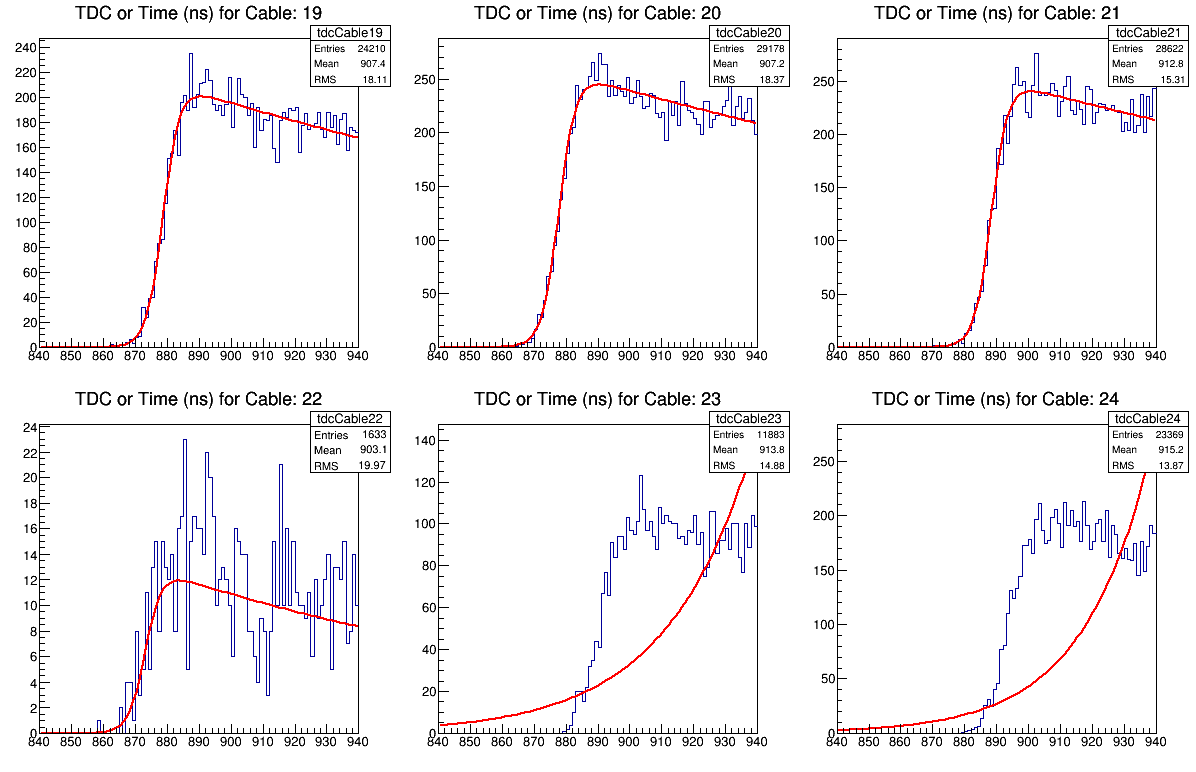
\includegraphics[width=3.0in]{Figures/tdcForRun085_Cables19to24.png}
    %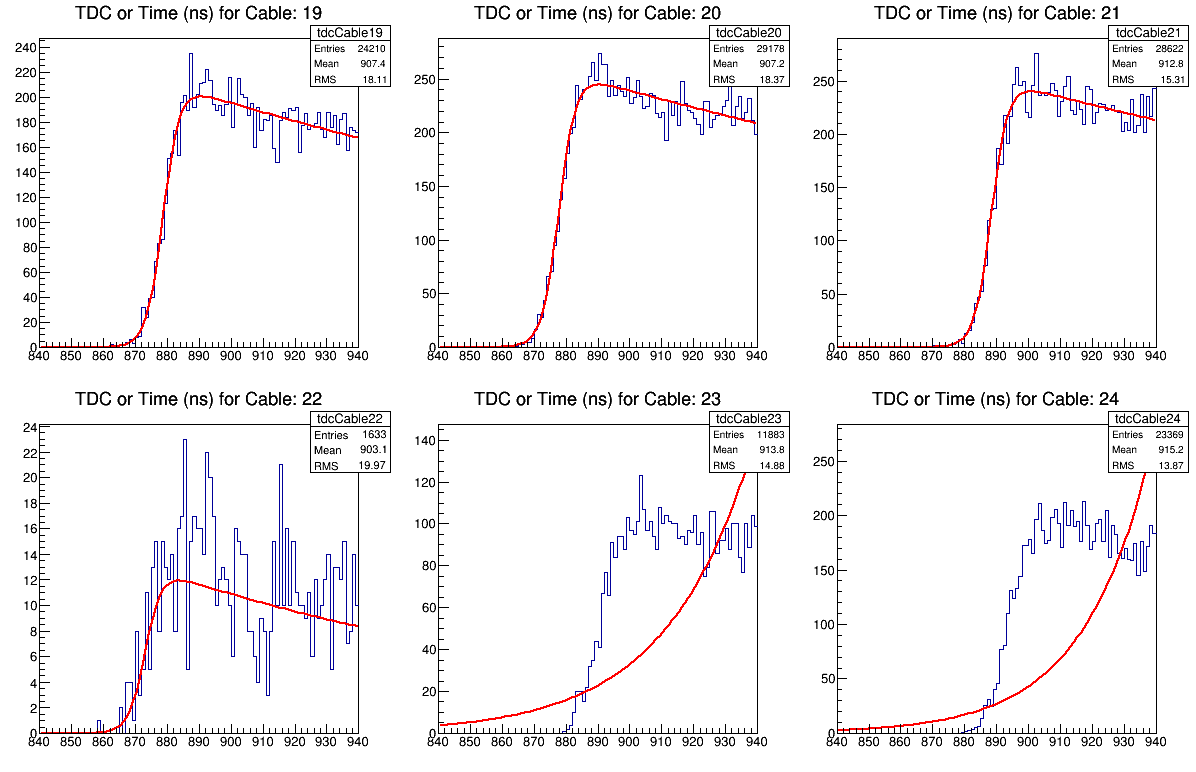
\includegraphics[scale=1.0]{Figures/tdcForRun085_Cables19to24.png}
    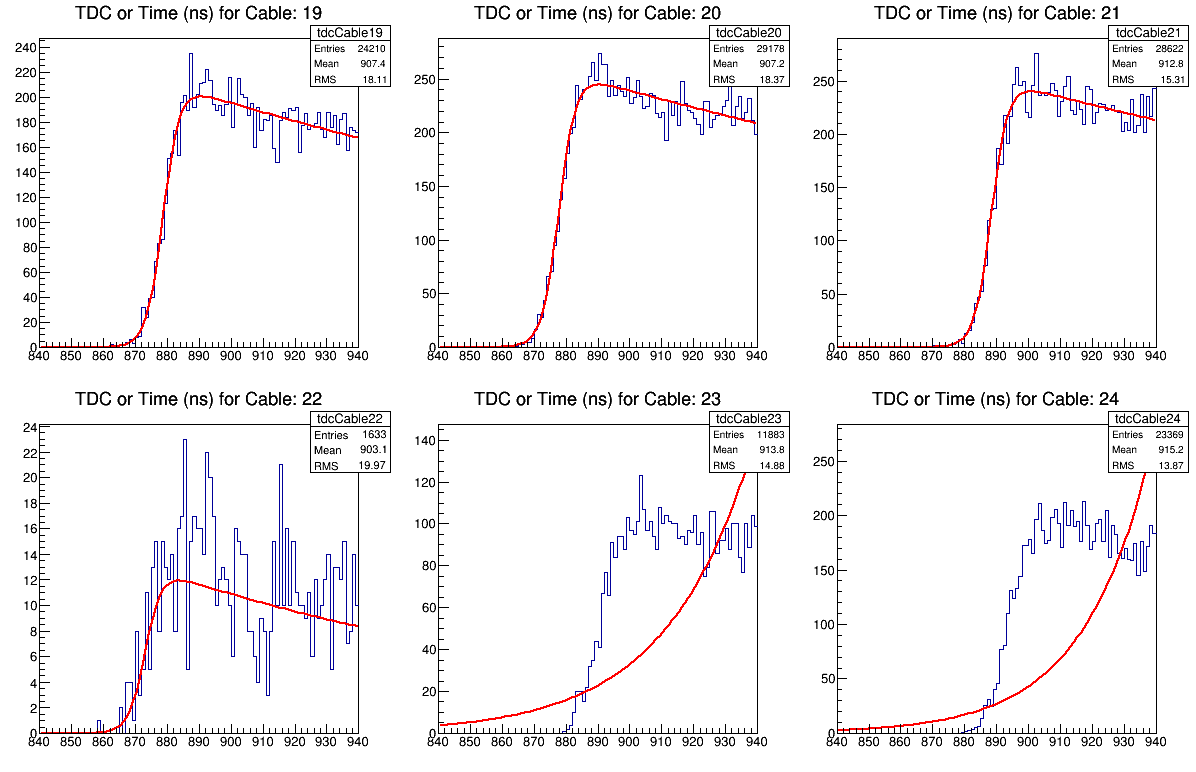
\includegraphics[width=1.0\textwidth]{Figures/tdcForRun085_Cables19to24.png}
    \caption{Time distributions showing fits when par[1] wasn't constrained well.}
    \label{tdcPosExp}
\end{figure}

\begin{figure}
    \centering
    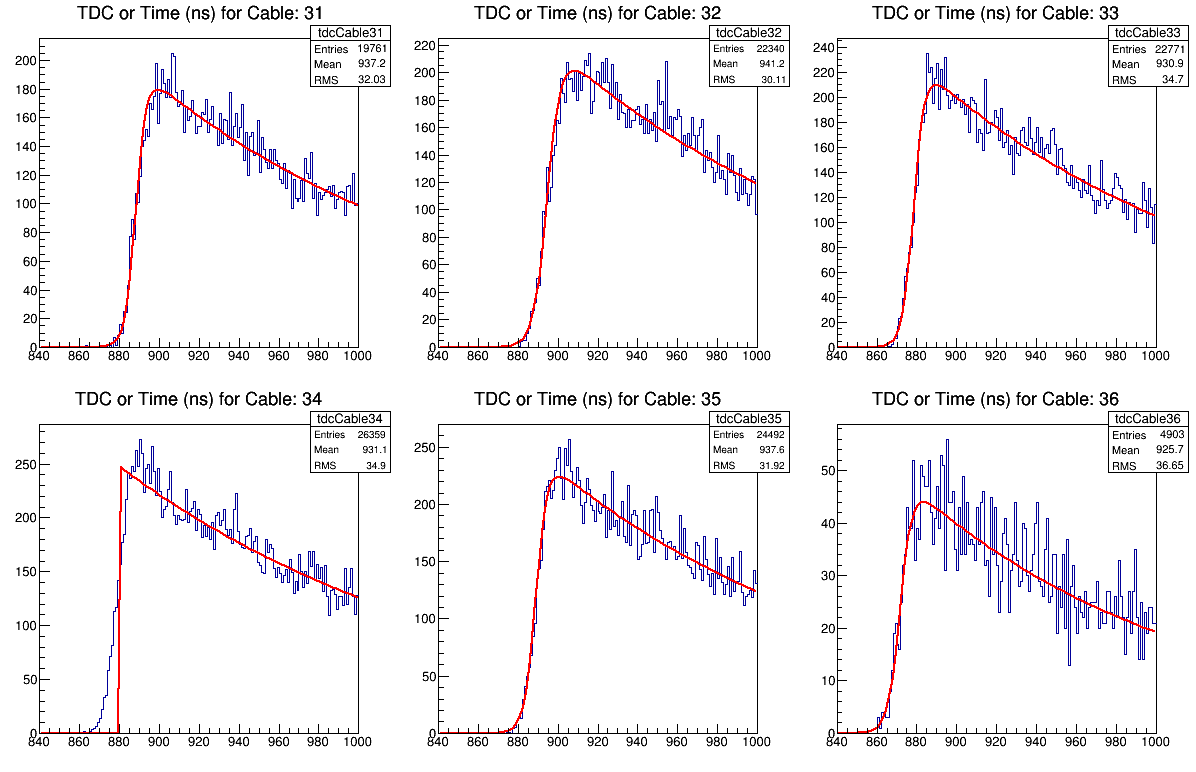
\includegraphics[width=1.0\textwidth]{Figures/tdcForRun068_Cables31to36.png}
    \caption{Time distributions showing fits when par[1] wasn't constrained well.}
    \label{tdcSharp}
\end{figure}


\subsubsection{Constraining par[4]}
And, without a limit on par[4] for the constant noise, sometimes it went negative (as big 
as 1480 - such as for 81st cable in figure \ref{tdcNegNoise}.
%in this set https://www.jlab.org/Hall-B//secure/eg4/adhikari/PDWK/CLAS12/BkUp/tdcForRun068_Cables79to84.gif . 
To avoid that situation, the parameter was allowed to vary only above zero and within [0.0,1.0e06].

\begin{figure}
    \centering
    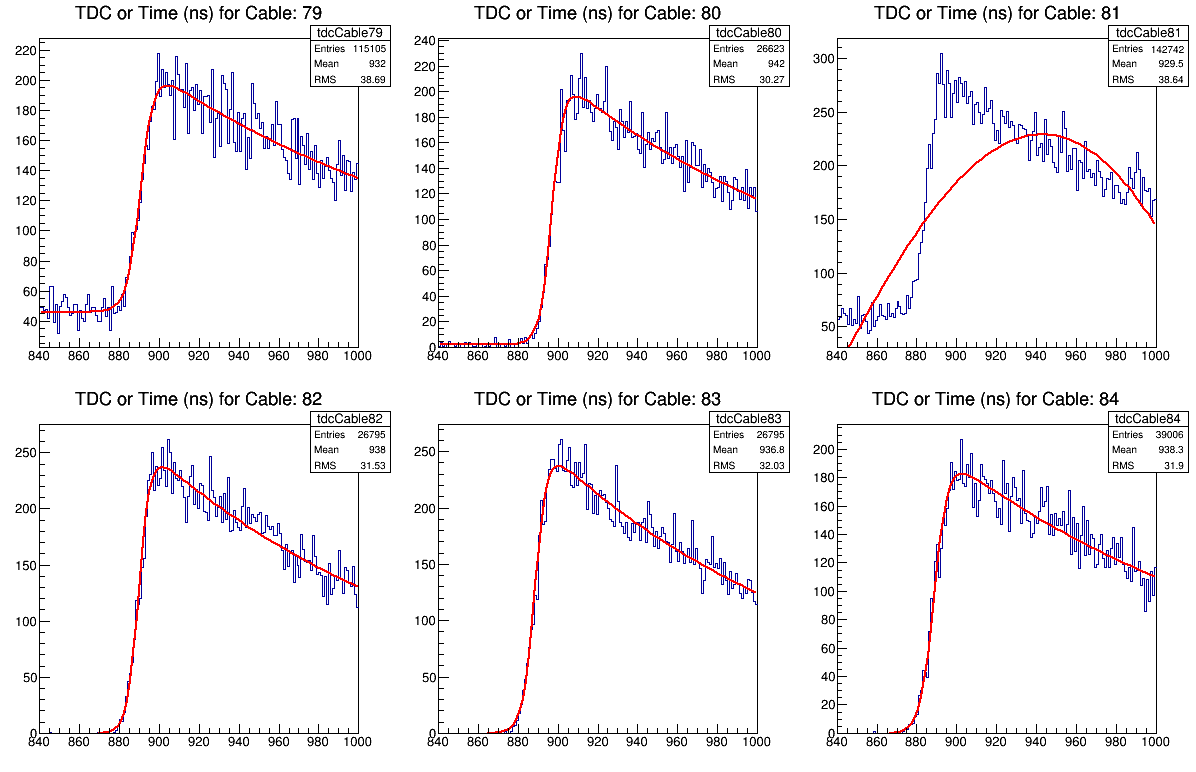
\includegraphics[width=1.0\textwidth]{Figures/tdcForRun068_Cables79to84.png}
    \caption{Time distributions showing fits when par[4] wasn't constrained well.}
    \label{tdcNegNoise}
\end{figure}


\subsubsection{Constraining par[2] and par[3]}

Next the cable 52 showed a little abnormal fit as seen in figure \ref{tdcSharp2}
%in https://www.jlab.org/Hall-B//secure/eg4/adhikari/PDWK/CLAS12/BkUp/tdcForRun068_Cables49to54.gif . 
When checked the values of the fit parameters, the value of par[2] was seen to be 1.82085e+04,
whereas in other cables, it was of the order of 3.0e+2. So, it was imperative to put 
limits on its value, which was chosen to be [100.0,4.0e02]. With that limit, the issue
was resolved, but it created a new problem in Cable 8 as reflected in figure \ref{tdcFlatFit}
%(https://www.jlab.org/Hall-B//secure/eg4/adhikari/PDWK/CLAS12/BkUp/tdcForRun068_Cables07to12.gif).
When checked again, it was that it had gotten  par[1]=-3.50957e-06 and par[2]=2.18599e+01. 
In other working cases, these values were of the order of -7.00443e-03 and 3.19779e+02, so 
the upper limit of par[1] above was changed from 0 to -1.0e-04. This made it better but 
still not quite as good as we wanted. Upon checking parameters again, it was seen that par[3] 
was of the order of -4.26634e-02 and par[2] of the order 3.80025e+01, whereas in the working case 
they were of order 2.83977e+02 and  -3.18337e-01. Therefore, par[2], and par[3] were also 
constrained within [100.0,4.0e02] and [-1.0,-1.0e-01] respectively.

\begin{figure}
    \centering
    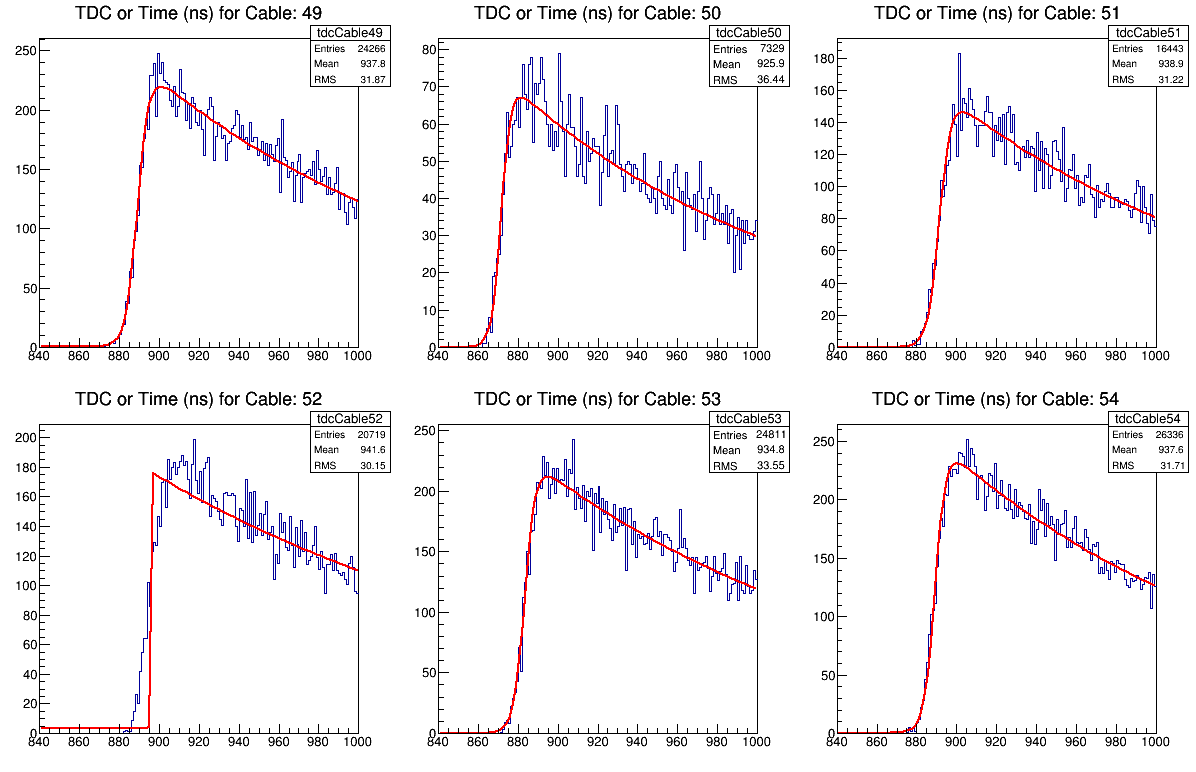
\includegraphics[width=1.0\textwidth]{Figures/tdcForRun068_Cables49to54.png}
    \caption{Time distributions showing fits when par[2] wasn't constrained well.}
    \label{tdcSharp2}
\end{figure}

\begin{figure}
    \centering
    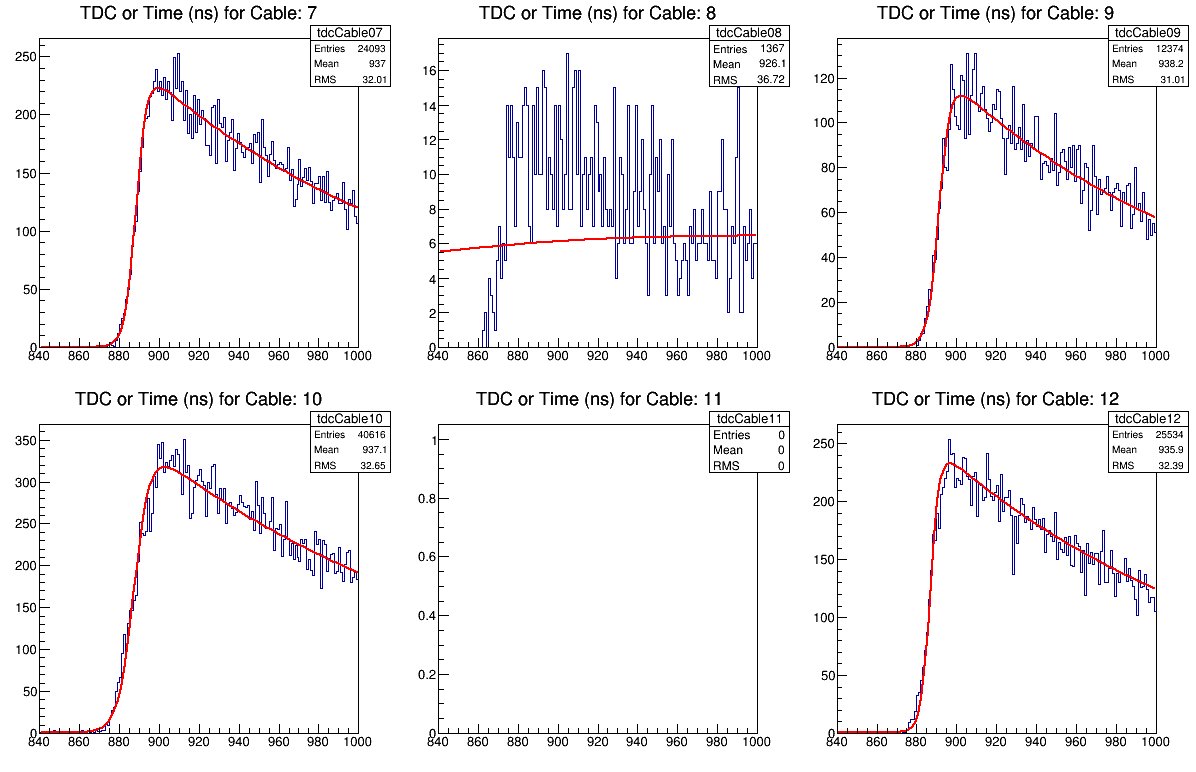
\includegraphics[width=1.0\textwidth]{Figures/tdcForRun068_Cables07to12.png}
    \caption{Time distributions showing fits when par[2] wasn't constrained well.}
    \label{tdcFlatFit}
\end{figure}



\subsubsection{Constraining par[0]}
Finally, to avoid getting cases such as that for cable 81 in figure \ref{tdcNoSigm}, 
%//https://www.jlab.org/Hall-B//secure/eg4/adhikari/PDWK/CLAS12/BkUp/tdcForRun068_Cables79to84nw0.gif
in which case par[0] was negative i.e, -1.09872e+01, the par[0] was also constrained inside [8.6,13.2].
\begin{figure}
    \centering
    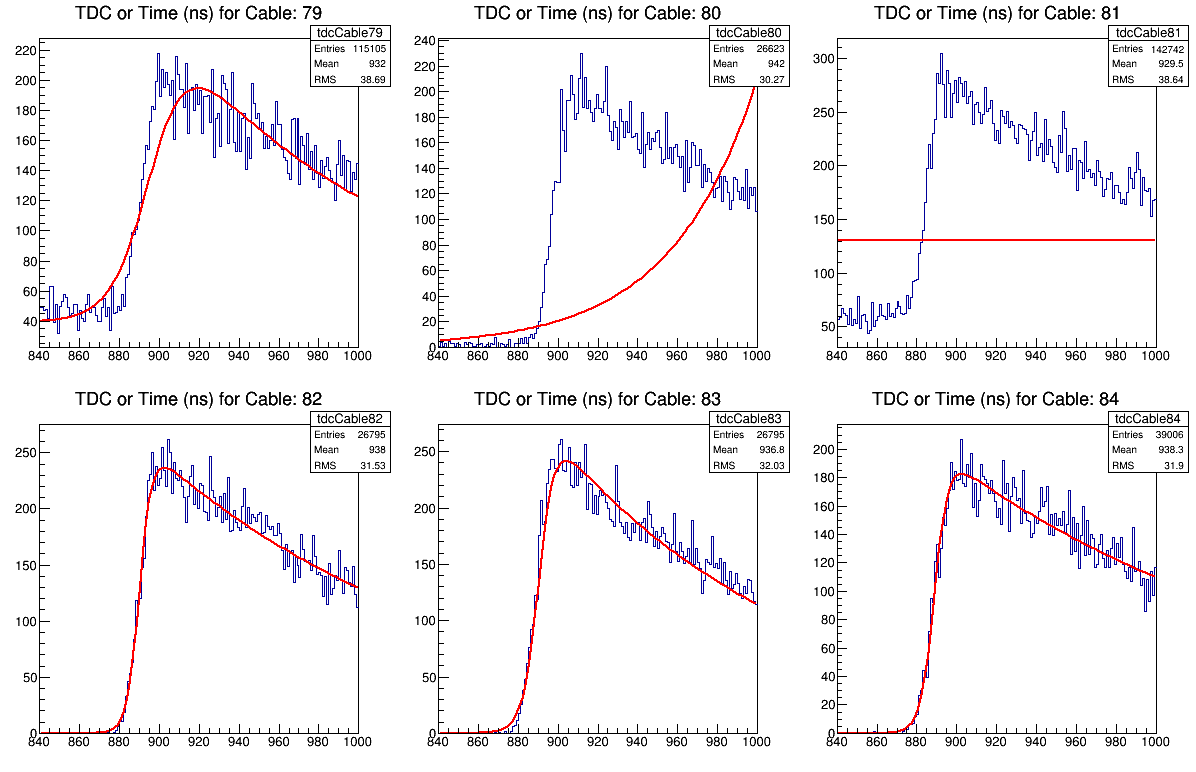
\includegraphics[width=1.0\textwidth]{Figures/tdcForRun068_Cables79to84nw0.png}
    \caption{Time distributions showing fits when par[0] wasn't constrained well.}
    \label{tdcNoSigm}
\end{figure}




\subsection{Estimating T0 values from the fits}

Once the overall fit is obtained, using the fit parameters $p_2$ and $p_3$, the sigmoid
function is singled out (extracted). Since the rising edge of the sigmoid fits well with the rising
edge of the TDC distribution, we can extract from this sigmoid the straight line that
represents the edge (i.e, the line with the same slope as the sigmoid at the half-way
point) as follows:

%\begin{comment}
\begin{eqnarray}
  \label{sigmEdge}
  y = slope*x + yIntercept 
\end{eqnarray}
%\end{comment}
where,
\begin{subequations}
\label{sig_mc}
\begin{eqnarray}
\label{sig_m}
%%//Slope of sigmoid = Derivative of 1/(1+exp(a+bx)) = -b*exp(a+bx)/(1 + exp(a+bx))^2
%%//derivSigHalfPoint = -fPars[3]*expAplusBx / pow((1.0+expAplusBx),2); //This is the slope of sigmoid at halfway point.
%%    derivSigHalfPoint = fa2->Derivative(sigmoidHalfwayPoint);
%%    funcValAtSigHalf = fa2->Eval(sigmoidHalfwayPoint);
slope = m = derivative of sigmoid = - p_3 \frac{e^{p_2 + p_3t}}{(1 + e^{p_2 + p_3t})^2} 
\end{eqnarray}

\begin{eqnarray}
\label{sig_c}
yIntercept  = ..
\end{eqnarray}
\end{subequations}

Although, we can evaluate  derivative analytically using above formula, in ROOT, we can do so by calling 
the Derivative method for the given function that represents the overall fit. Thus, at the half-way point, the 
derivative or the slope would be given as follows:

\begin{eqnarray}
\label{fSlopeAt1By2}
slope = m = fitFunc->Derivative(sigmoidHalfwayPoint);
\end{eqnarray}

Likewise, the value of the fit function at the same sigmoid-halfway-point is given as follows:

\begin{eqnarray}
\label{fValAt1By2}
funcValAtSigHalf = fitFunc->Eval(sigmoidHalfwayPoint);
\end{eqnarray}

where $sigmoidHalfwayPoint = |par[2]/par[3]|$ (modulus is for the fact that the ratio is 
$par[2]/par[3]$ negative due to par[3] being constrained to negative values (see 
table \ref{tabParLimits}).



With that, now we can make two different estimates of T0 as described below. The first estimate
is by extrapolating the straight line (which represents the slope) down to the level of the noise background (== par[4]) 
and finding out the corresponding value along the X- or T-axis.
\begin{equation}
\label{T0estm1}
\begin{aligned}
%//X value where the st. line meets the noise background (background = fPars[4] (Extrapolation upto noise level)
   T0   = & sigmoidHalfwayPoint + \\
          & \frac{1}{derivSigHalfPoint} (par[4] - funcValAtSigHalf); 
\end{aligned}
\end{equation}



The second method is extrapolating the same straight line further down such that the corresponding value of
time where it meets the time-axis gives us the T0 estimate as follows:
\begin{equation}
\label{T0estm2}
\begin{aligned}
%//X value where the st. line meets the X or time axis (Extrapolation upto  y=0 level i.e upto X or time axis)
   T0  =    &  sigmoidHalfwayPoint + \\
            & \frac{1}{derivSigHalfPoint} (0.0 - funcValAtSigHalf);
\end{aligned}
\end{equation}


\begin{comment}
%http://tex.stackexchange.com/questions/8936/how-to-break-a-long-equation 
\begin{equation}
\begin{aligned}
F   ={} & \{F_{x} \in  F_{c} : (|S| > |C|) \\
        & \cap (\mathrm{minPixels}  < |S| < \mathrm{maxPixels}) \\
        & \cap (|S_{\mathrm{conected}}| > |S| - \epsilon)\}
\end{aligned}
\end{equation}
\end{comment}




\section{Procedure for \tmax estimation}
To dermine the \tmax for a given cable, a histogram is made of the TDC values recorded for all the hits corresponding to the cable. Then towards the falling edge, the histogram is fit to the following function with five free parameters $p_0$, .., $p_4$.

%\begin{comment}
\begin{equation}
    \label{T0fit}
    f(t) = e^{p_0 + p_1t} (1 - \frac{1}{1 + e^{p_2 + p_3t}})  + p_4
    % f(t) = exp*sigmoid + constant
    %   exp: decaying behaviour after the rising edge
    % sigmoid: for the S-shape of the signal
    % constant: for the noise in data for some cables.
\end{equation}
%\end{comment}

where $(1 - \frac{1}{1 + e^{p_2 + p_3t}})$ can be called as the inverse-sigmoid.


\subsection{Parameter Constraints}



\subsection{Estimation of \tmax}

When the values of the parameters are determined by the fits, the corresponding inverse-sigmoids 
can be extracted, from which a straight line fit to the falling edge at its half-way point ($sigmoidHalfwayPoint$)
can be determined. By extrapolating this straigh line, \tmax can be determined.

Here, $sigmoidHalfwayPoint = |par[2]/par[3]|$ (modulus is for the fact that the ratio is 
$par[2]/par[3]$ negative due to par[3] being constrained to negative values (see 
table \ref{tabParLimits}).



\section{Conclusion}



\end{document}
